% igs2ejournalguide.tex
% v4.00 3-sept-2015

\NeedsTeXFormat{LaTeX2e}

% check that the math fits the two-column format:
% \documentclass[twocolumn]{igs}

% but use this version when submitting your article:
  \documentclass[review,oneside]{igs}

% other options are available
%   authors printing on US letter size are advised 
%   to use the slightly shorter [letterpaper] option
% SINGLE COLUMN
%   \documentclass{igs}              
% SINGLE COLUMN, FEWER LINES/PAGE
%   \documentclass[letterpaper]{igs} 
% DOUBLE COLUMN, FEWER LINES/PAGE
%   \documentclass[twocolumn,letterpaper]{igs} 

  \usepackage{igsnatbib}

% check if we are compiling under latex or pdflatex
  \ifx\pdftexversion\undefined
    \usepackage[dvips]{graphicx}
  \else
    \usepackage[pdftex]{graphicx}
    \usepackage{epstopdf}
    \epstopdfsetup{suffix=}
  \fi

% the default is for unnumbered section heads
% if you really must have numbered sections, remove
% the % from the beginning of the following command
% and insert the level of sections you wish to be
% numbered (up to 4):

% \setcounter{secnumdepth}{2}

\begin{document}

\title[GRACE Forward Modeling]{GRACE forward modeling of Gulf of Alaska water balances}

\author[Arendt and others]{ }

%\affiliation{%
%$^1$Applied Physics Laboratory, University of Washington \\ E-mail: arendta@uw.edu \\ $^2$Planetary Geodynamics Laboratory, NASA Goddard Space Flight Center, Code 698, Greenbelt, MD, 20771\\ $^3$ School of Civil and Construction Engineering, Oregon State University, Corvallis, OR, 97331, USA}

\abstract{...}

\maketitle

\section{Introduction}

Data from the NASA/DLR Gravity Recovery and Climate Experiment (GRACE) have been fundamental tools for assessing mass variations of alpine and high latitude regions \citep{wouters_grace_2014}. To date, much research has focused on the ice sheets, where the uniformity of land cover type minimizes the number of different geophysical signals that need to be partitioned in GRACE processing \citep{shepherd_reconciled_2012}. In contrast, non-ice sheet (mountain glacier) regions usually exist within a dispersed mixture of land and ocean cover types that often include complex fjords, coastal temperate rainforests, lakes, rivers and seasonal snowpacks, making it difficult to partition the collection of hydrological and geophysical signals that GRACE observes. The problem is compounded by the fact that many non-glacier surfaces have semi-annual periodicity in their mass fluctuation that mimic those of glaciers. Because of these complexities, Most GRACE mountain glacier studies have focused on recovering the cumulative change in mass \citep{reager_decade_2016} where glacier volume loss signals are assumed to be the dominant driver of changes in hydrological storage. Nevertheless, there is a need for full utilization of the sub-annual components of the GRACE signal to inform studies of water resource availability, impacts of freshwater discharge on ecosystem services, and predicting the likelihood of runoff-related hazards \citep{oneel_icefield--ocean_2015}.

Nearly all GRACE studies aim to isolate a mass change signal of interest as a residual of GRACE processing after all other systems have been accounted for through observations or models. In the case of mountain glacier studies, models such as the Global Land Data Assimilation System (GLDAS, \citep{rodell_global_2004}) are used to remove all non-glacier sources of hydrological variations. Within GLDAS are land surface hydrology models such as the Community Land Model \citep{oleson2010technical} and the Variable Infiltration Capacity model \citep{liang1994simple}. At mid- to low latitudes, the accuracy of such models is generally good \citep[e.g.][]{werth_integration_2009}. However at high elevation and latitude, these models are limited in their capacity to fully account for changes in terrestrial snowpack, groundwater storage, lake level fluctuations and precipitation. The primary problem is that such models do no have paramaterizations for glacier ice flow, and therefore any solid precipitation that is not removed in a given season can accumulate indefinitely on high elevation grid cells. To account for this, all GRACE studies to date have simply eliminated land surface hydrology corrections from those grid cells containing glacier ice \citep[e.g.][]{gardner_sharply_2011,jacob_recent_2012,luthcke_antarctica_2013}. Due to the relatively coarse resolution of the land surface hydrology models (generally >25 km), this correction procedure removes significant non-glacier areas from the analysis, leading to errors and mis-attribution of signal. An additional complication relates to the periodicity of mass change signals relative to the period of GRACE processing. Aliasing of daily, multi- and sub-daily cycling in hydrological signals occurs when these signals are averaged over monthly time scales and then removed from fully processed GRACE solutions. Additional computations are also necessary to properly compare hydrological observations collected at discrete points in time with time-averaged monthly values acquired from multiple GRACE measurements over a particular region \citep{swenson_estimating_2006,hill_spatial_2015}. 

An alternative approach to partitioning GRACE signals involves 

creating best estimates of the mass variations in the signal of interest are developed from independent models \citep{beamer_high-resolution_2016}, datasets \citep{sasgen_towards_2012}, or random algorithms \citep{gardner_sharply_2011,colgan_constraining_2013}. The simulated signal is then forward modeled to a degree and order that match GRACE resolution, and the observed and simulated GRACE signals are compared. Joint inversion of GRACE together with GPS/ocean bottom pressure \citep{wu_simultaneous_2010} and sea surface height \citep{jensen_land_2013} have been used to provide additional constraints that help minimize uncertainty in attribution of the GRACE signal. All of these studies aim to better isolate the spatial and temporal patterns in mass change of regions with complex hydrology. By forward modeling and using inversion or Monte Carlo methods, they minimize uncertainties that result from smoothing and filtering when removing signal from a fully processed GRACE solution.

Despite this progress in method development, there are several limitations to the above approaches. The first is that independent datasets used to initialize forward modeling studies have focused on glacier volume loss \citep[e.g.][]{sasgen_towards_2012}, i.e. the long-term trend in the GRACE signal. Seasonal changes have been entirely attributed to glacier seasonal mass balances, with limited consideration of the role of terrestrial snowpack and other annually-varying components of the system. The second is that the random generation of a synthetic mass change curve makes it impossible to understand partitioning of mass changes among various hydrological systems. While the full signal may be well captured by such approaches, it returns a bulk measure of mass change with no knowledge about the individual source contributors. The third problem is that the spatial resolution of existing inversion/forward modeling approaches is on the scale of large watersheds, limiting our ability to use GRACE to understand processes at smaller spatial scales.

The watersheds bordering the Gulf of Alaska (GOA) presently discharge approximately 850 km$^3$ yr$^{-1}$ \citep{hill_spatial_2015} of freshwater to the ocean, and as such are an excellent case study for developing new approaches for processing GRACE. Seasonal and multi-annual variations in these runoff volumes have impacts on near shore ecosystems and ocean circulation patterns \citep{oneel_icefield--ocean_2015}. Using a fully distributed energy balance model at 1 km resolution, \cite{beamer_high-resolution_2016} have shown that the partitioning of GOA runoff between snow melt, glacier ice melt and rainfall during 2002-2014 was 63\%, 17\% and 20\% respectively. 

% Data from the Gravity Recovery and Climate Experiment (GRACE) have been used to assess the hydrology of the GOA region. Early work focused on recovering the trends in mass from GRACE to assess Glacier Volume Loss (GVL) \citep{sasgen_towards_2012,schrama_mascon_2014,harig_ice_2016,reager_decade_2016}. 



\citep{lenaerts_irreversible_2013}

\section{Methods}

The GRACE mission has revolutionized our ability to monitor global water mass variability by mapping the Earth’s gravity field each month with a spatial resolution of 300-400 km. Applying GRACE solutions to high-resolution studies, however, poses significant challenges. Due to large increases in the GRACE gravity errors at small spatial scales, the project spherical harmonic solutions must be filtered prior to their application to geophysical research. GRACE mascon estimation, initially developed by the gravity group at NASA Goddard Space Flight Center (GSFC) [Rowlands, 2005; Sabaka et al., 2010; Luthcke et al., 2013], is quickly becoming the preferred method for time-variable gravity estimation (e.g. [Watkins et al., 2015]). The mascon approach optimizes the solution signal to noise ratio by introducing a geophysical-based regularization matrix in the normal equations, providing a great benefit to researchers who no longer need to design and apply a post-processing filter to the GRACE solutions. However, the mascons still exhibit the same fundamental spatial resolution as the spherical harmonics within a mascon constraint region. Attempts to overcome the resolution limits of GRACE have been made with the estimation and application of 1x1 equal-angle gain factors using a combination of Terrestrial Water Storage (TWS) models and filtered GRACE solutions [Landerer and Swenson, 2012]. The main deficiency in this approach is the significant information loss that occurs when filtering GRACE solutions to their fundamental resolution. Even though this scaled GRACE TWS product is distributed at 1×1 (Figure 1), it should only be analyzed after combining a sufficient number of grid cells to form regions large enough to be resolved by GRACE.

These limitations in the spatial resolution of GRACE motivated the development of a forward modeling approach. The conceptual benefit of forward modeling is simple: by accounting for as much of the known mass variability in the Level 1B (i.e. the intersatellite range rate measurements) processing as possible, the magnitude of the inter-satellite residuals and updates to the gravity field are minimized. This approach reduces the well-known problem of temporal aliasing and limits the portion of the estimated gravity field that is subject to the fundamental spatial resolution of the GRACE-determined solutions. In the case of a perfect forward model, the Level 1B processing would produce inter-satellite ranging measurement residuals of zero (ignoring the effects of noise and systematic errors), and no updates to the gravity field would be made. It is important to note that though GRACE solutions are limited in their ability to spatially resolve signals, the Level 1B inter-satellite measurements are in fact sensitive to high temporal and spatial resolution variability, and unmodeled signals of sufficient magnitude at any resolution will manifest as non-zero updates to the mascons.

Since the beginning of the mission, GRACE Level 1B processing centers have relied on forward modeling to remove the effects of ocean tides, atmospheric, and non-tidal ocean mass variability. [Sabaka et al., 2010] demonstrated the benefit of also including a TWS model for the further reduction of the inter-satellite measurement residuals and the mitigation of signal leakage into or out of regions of hydrologic variability. Luthcke et al. [2013] expanded this idea further with the implementation of a fully iterated time-variable mascon solution, where each iterative solution defines the forward model for the subsequent iteration, demonstrating a simultaneous increase in signal and decrease in residual magnitude until solution convergence occurred. In addition to the typical forward models listed above, the current NASA GSFC global mascon solution also models TWS from Global Land Data Assimilation (GLDAS)/Noah [Rodell et al., 2004], ICE-6G glacial isostatic adjustment (GIA) [Peltier et al., 2015], and the largest co-seismic events [Han et al., 2013]. Our proposal will leverage the Level 1B processing and global mascon estimation capabilities at NASA GSFC, resulting in monthly estimates of 41,168 1×1 arc-degree equal-area cells in terms of cm of equivalent water height. As previously discussed, the true resolution of the solution (300 km) is lower than that of the equal-area mascon grid (≈111 km), but the higher resolution mascon definition allows for a more accurate representation of the land/ocean boundaries that define the constraint regions, across which mascons are
uncorrelated.

The forward model approach in the context of this study is as follows: GMELT datasets and models of mass changes of the HMA (Figure 2) will define the high-resolution model in the HMA region while the rest of the global model is the NASA GSFC GRACE mascon solution (all other previously described components of the NASA GSFC forward model procedure are also included). Time series of mass changes from GMELT will be combined into an ensemble product based on consensus across the HiMAT team. We will explore the use of weighting factors to combine multiple overlapping estimates, or the testing of different data/model combinations within our iterative framework. Next or best estimates will be expressed to at least spherical harmonic degree and order 90, where the expansion size can be increased if it is determined to be beneficial. Each new Level 1B processing produces a new global mascon solution, where the HMA region mascons describe the long spatial wavelength GMELT error, which serves as feedback for the next iterative construction of the GMELT water balances. Updated GMELT model output is iteratively applied to new Level 1B forward model runs until the GRACE mascon updates are sufficiently close to zero, indicating that the high-resolution GMELT model is in full agreement with the GRACE measurements. It may prove to be more effective and efficient to circumvent the formation and inversion of normal equations by directly analyzing the range-rate or range-acceleration residuals generated from the Level 1B processing as described in recent studies [Loomis et al., 2015; Eicker and Springer, 2016]. We note that our iterative procedure enables adjustment of parameters on individual modules of GMELT, or on weighting factors that combine the ensemble of mass change estimates.

NASA GSFC GRACE Level 1B processing applies a baseline orbit parameterization [Rowlands et al., 2002] that does not require the processing and reduction of GPS measurements, but instead uses the GPS-determined Level 1B navigation files to define the initial orbit that is adjusted simultaneously with the gravity from the inter-satellite measurements (also accounting for the Level 1B attitude quaternions and accelerometer measurements). This allows for the rapid formation and inversion of normal equations for the full duration of the GRACE mission. The ability to quickly process and invert new solutions is an important practical consideration for the work proposed here, where a number of different GMELT outputs will need to be analyzed and iterated.

\section{Discussion}

\section{Acknowledgements}

Support for this work was provided by NASA under the GRACE Science Team, Interdisciplinary Science (IDS) and Cryospheric Sciences program (grant NNH07ZDA001N-CRYO). We gratefully acknowledge the quality of the Level-1B products produced by our colleagues at the Jet Propulsion Laboratory. We especially thank J.P. Boy and R. Ray for their contributions to the forward models used in this study. 

\bibliography{c:/work/glaciology}
%\bibliography{igsrefs}
\bibliographystyle{igs}

%\begin{SCfigure}
%\centering
%\caption{Geophysical signals measured by GRACE satellites over mountainous terrain include glacier mass balance ($\Delta M_{glaciers}$), changes in lake, groundwater and non-glacier snowpack ($\Delta M_{TWS}$), atmospheric mass ($\Delta M_{atmosphere}$), ocean tides ($\Delta M_{ocean}$) and the viscoelastic component of isostatic uplift ($\Delta M_{mantle}$).} 
%\includegraphics[width=0.7\textwidth]{GRACE_system}
%\label{fig:system}
%\end{SCfigure}


\begin{figure}[h]
\noindent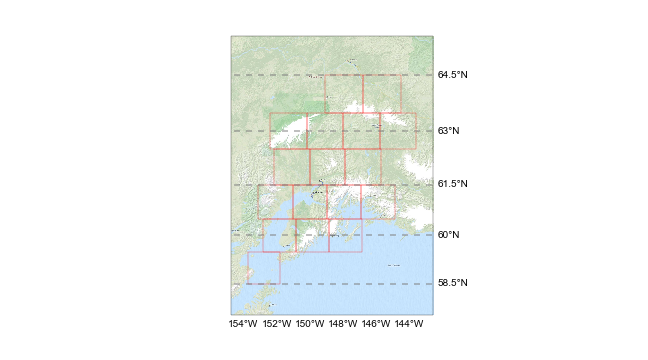
\includegraphics[width=178mm]{figures/westernMap} \centering \caption{Mascons of the western Gulf of Alaska.} \label{fig:wGOA_map}
\end{figure}

\begin{figure}
\noindent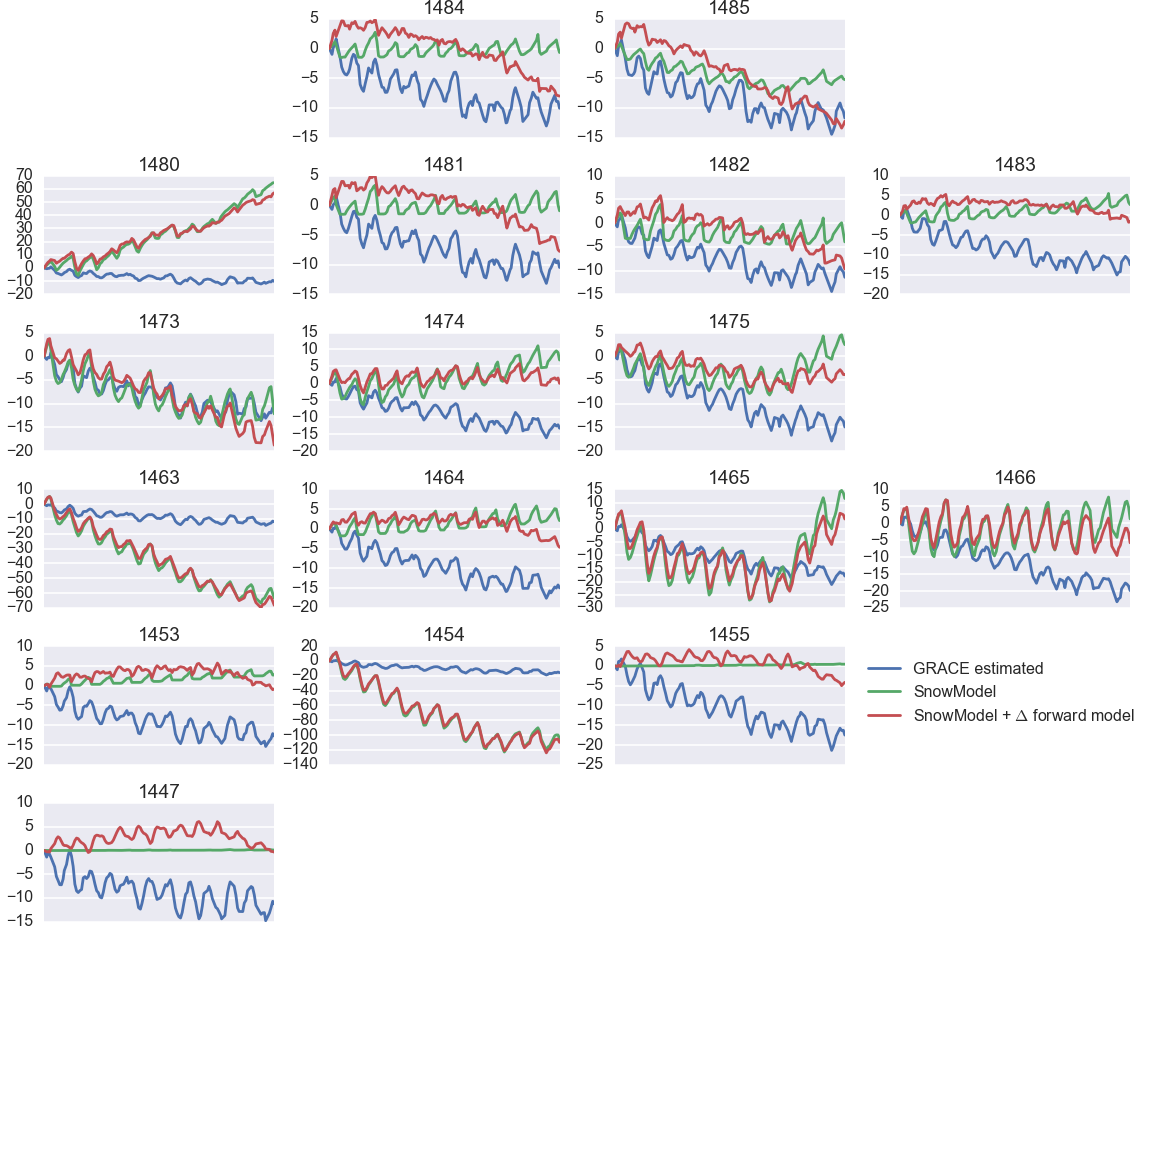
\includegraphics[width=178mm]{figures/westernPlot} \centering \caption{Comparison of GRACE water balances prior to forward modeling \citep{luthcke_antarctica_2013}, (blue); modeled water balances using SnowModel \citep{beamer_high-resolution_2016} (green); and modeled water balance corrected by the forward modeling in this study (red). Subplots are arranged to approximately match the geographic layout of thier respective mascons in Fig. \ref{fig:wGOA_map}} \label{fig:wGOA_plot}
\end{figure}

\begin{figure}
\noindent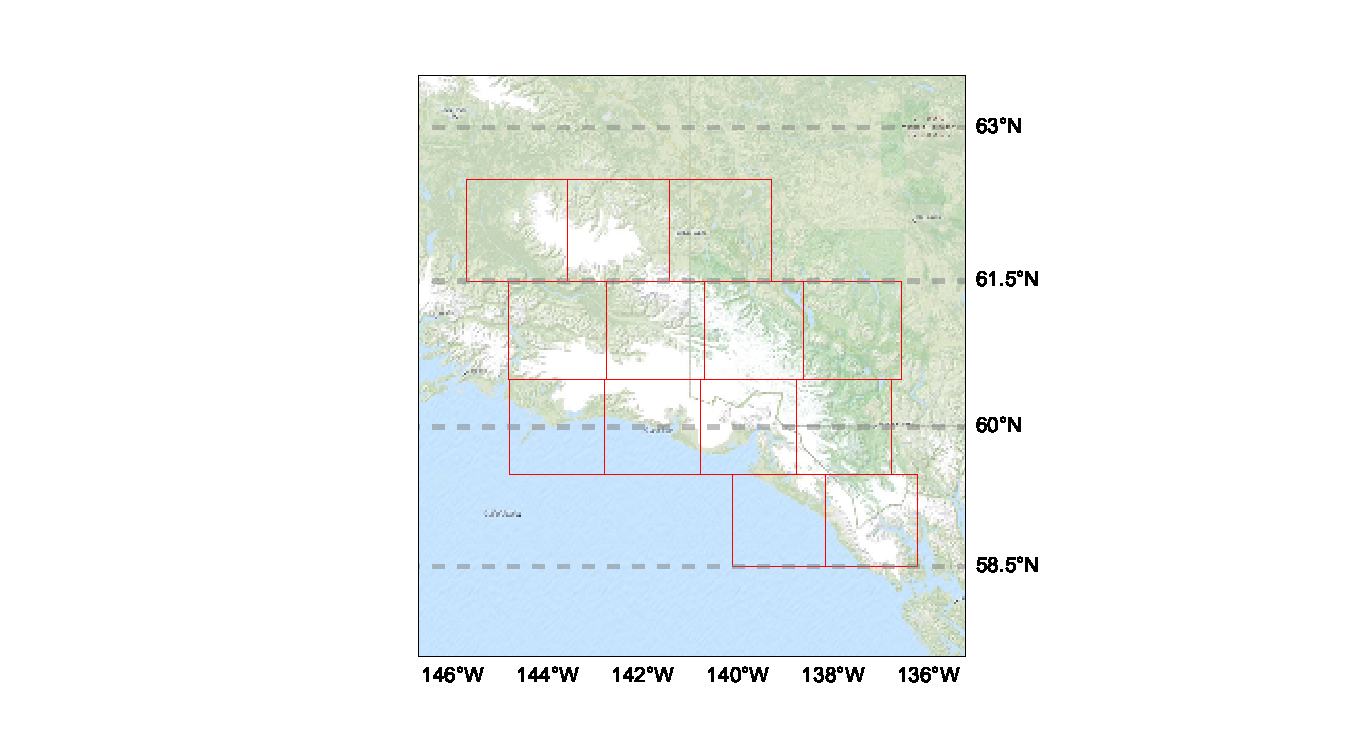
\includegraphics[width=178mm]{figures/easternMap} \centering \caption{Mascons of the western GOA} \label{fig:summer}
\end{figure}

\begin{figure}
\noindent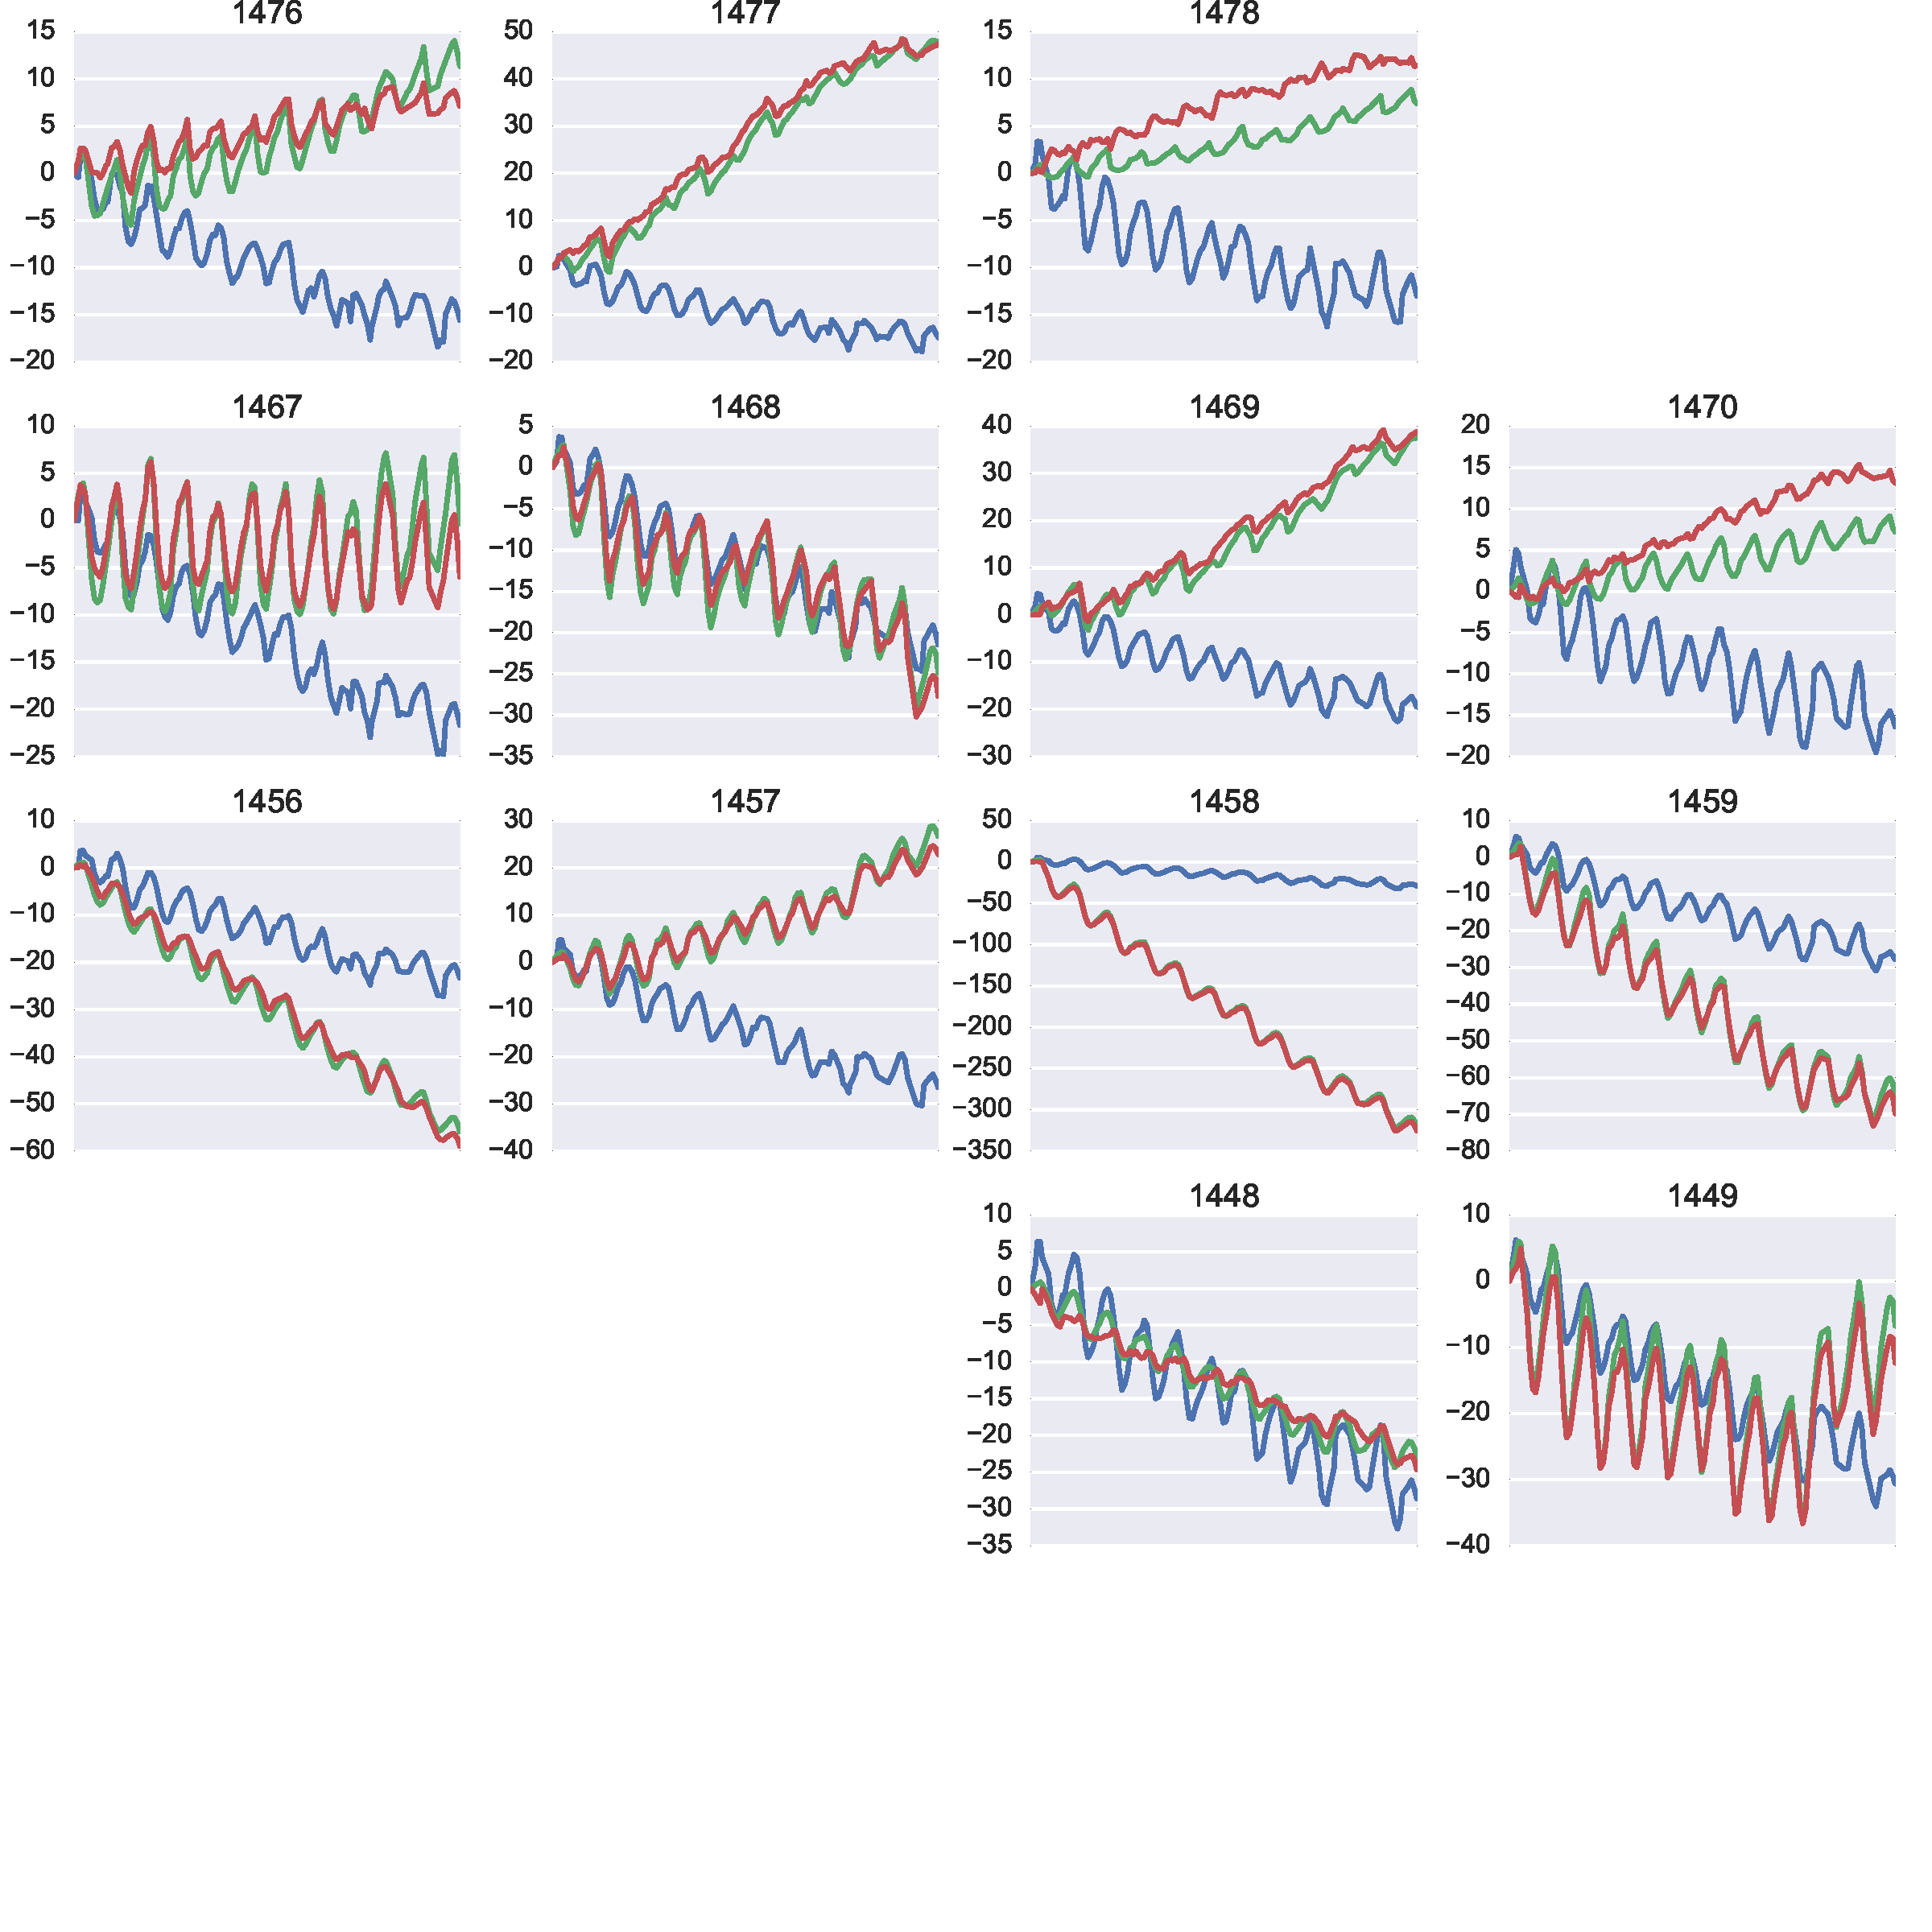
\includegraphics[width=178mm]{figures/easternPlot} \centering \caption{Mascons of the western GOA} \label{fig:summer}
\end{figure}


\begin{figure}
\noindent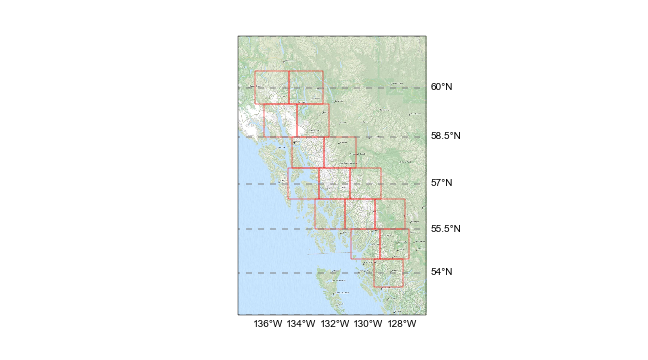
\includegraphics[width=178mm]{figures/southeasternMap} \centering \caption{Mascons of the western GOA} \label{fig:summer}
\end{figure}

\begin{figure}
\noindent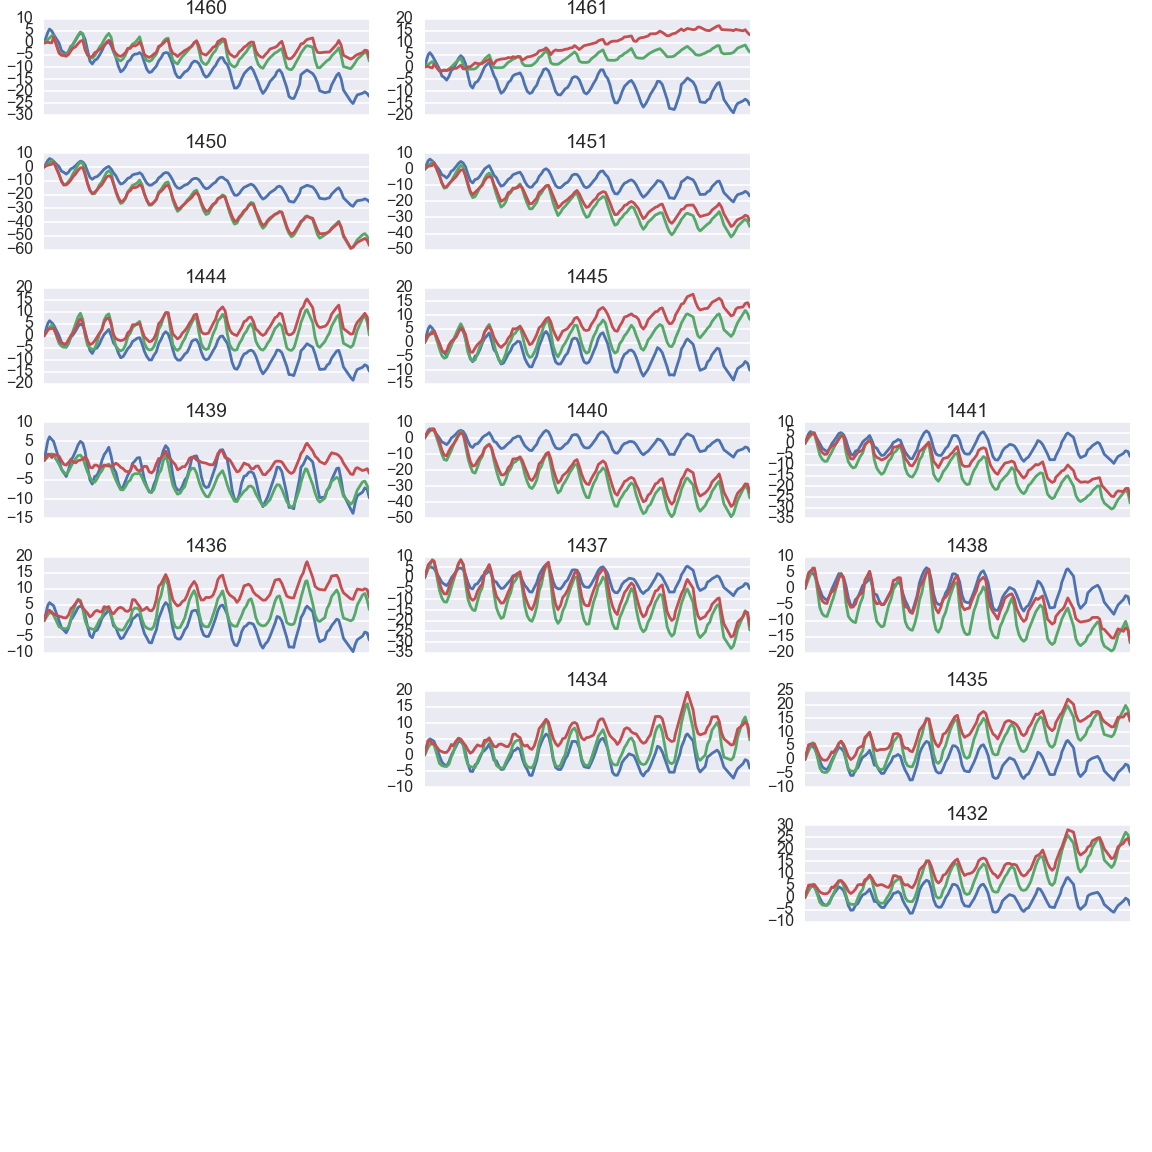
\includegraphics[width=178mm]{figures/southeasternPlot} \centering \caption{Mascons of the western GOA} \label{fig:summer}
\end{figure}

% width = 86 mm
%\begin{figure}[h]
%\includegraphics[width=178mm]{figures/700mbTempDepart_lowres} \centering \caption{Departures in summer (June to August) 700 mb air temperature (mean of NCEP R-2 and ERA-40 reanalysis) from 2004-2010 mean at each of the eight GRACE mascon drainage systems.} \label{fig:upperAir}
%\end{figure}


\end{document}
